%\begin{frame}
%\only<1>{\frametitle{Simple RNN + memory state cells}}
%\only<2,3,4>{\frametitle{Simple RNN + memory state cells + input gates}}
%\only<5->{\frametitle{Simple RNN + memory state cells + input gates + output gates}}
   
%\only<1>{
%\begin{center}
	%\includegraphics<1>[width=0.8\textwidth]{img/lstm_delay_unroll_memory}
	%\notesonly{
	%\captionof{figure}{Adding memory state cells to the simple RNN unrolled in time.}
	%}
%\end{center}
%}
%\only<2,3,4>{
%\begin{center}
%\slidesonly{
	%\includegraphics<2>[width=0.8\textwidth]{img/lstm_delay_unroll_write_gate_only}
	%\includegraphics<3>[width=0.8\textwidth]{img/lstm_delay_unroll_write_connect}
%}
	%\includegraphics<4>[width=0.8\textwidth]{img/lstm_delay_unroll_write}
	%\notesonly{
	%\captionof{figure}{Adding input gates.}
	%}
%\end{center}
%}
%\only<5->{
%\begin{center}
	%\includegraphics<5>[width=0.7\textwidth]{img/lstm_delay_unroll_write_read_gate_only}
	%\includegraphics<6->[width=0.7\textwidth]{img/lstm_delay_unroll_write_read}
	%\notesonly{
	%\captionof{figure}{Adding input and output gates.}
	%}
%\end{center}
%}

%\mode<presentation>{
	%\svspace{-5mm}
	%\begin{eqnarray*}
		%\vec c^{(t)} &=& {\color{magenta}1.0}~\vec c^{(t-1)} 
				%+  {\color{blue} \visible<2->{ \vec g^{\mathrm{i}(t)} \odot}  \tanh\Big( 
					%\vec W^\mathrm{c} \vec s^{(t-1)} \Big)
					 %} \\[-1mm]
		%\vec y^{(t)} &=& f\Big( \vec V^\mathrm{y} \, \vec s^{(t)} + \vec b^\mathrm{y}
					%+ {\color{darkgreen} \vec U^\mathrm{y} 
					%\visible<6->{\big(} \vec c^{(t)} 
					%\visible<5->{\odot \vec g^{\mathrm{o}(t)} \big)} } 
					%\Big) \,,
					%\qquad \text{e.g.}\;f(\cdot)=\text{softmax}(\cdot) \\[-1mm]
		%\vec s^{(t)} &=& \tanh\Big( \vec U^\mathrm{h} \, \vec x^{(t)}  
				%+ \vec W^\mathrm{h} \, \vec s^{(t-1)} + \vec b^\mathrm{s}
				%+ {\color{darkgreen} \vec V^\mathrm{h} 
					%\visible<6->{\big(} \vec c^{(t-1)} 
					%\visible<5->{\odot \vec g^{\mathrm{o}(t)} \big)} }
				%\Big) \\[-1mm]
		%\visible<2->{\color{blue} \vec g^{\mathrm{i}(t)}} 
			%&\visible<2->{\color{blue}=}& 
			%\visible<3->{\color{blue}
				%\sigma\Big(\vec U^\mathrm{i} \, \vec x^{(t)} 
				%+ \vec V^\mathrm{i} \, \vec c^{(t-1)} 
				%+ \vec W^\mathrm{i} \, \vec s^{(t-1)} 
				%+ \vec b^\mathrm{i} \Big) } \\[-1mm]
		%\visible<5->{\color{darkgreen} \vec g^{\mathrm{o}(t)}} 
			%&\visible<5->{\color{darkgreen}=}& 
			%\visible<6->{\color{darkgreen}
				%\sigma\Big(\vec U^\mathrm{o} \, \vec x^{(t)} 
				%+ \vec V^\mathrm{o} \, \vec c^{(t-1)} 
				%+ \vec W^\mathrm{o} \, \vec s^{(t-1)} 
				%+ \vec b^\mathrm{o} \Big) } 
	%\end{eqnarray*}	
	%}

%\end{frame}

%\begin{frame}{Building an LSTM from an RNN}

%\mode<presentation>{
%\begin{center}
	%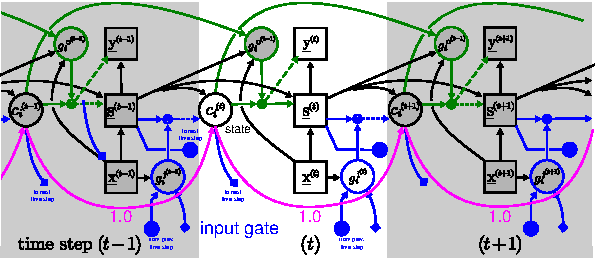
\includegraphics[width=0.7\textwidth]{img/lstm_delay_unroll_write_read}
%\end{center}

%\pause

%\begin{center}
	%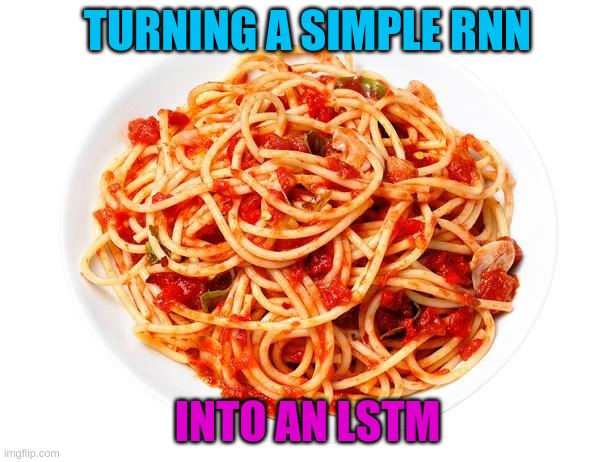
\includegraphics[width=0.4\textwidth]{img/meme_lstm_spaghetti}
%\end{center}
%}
%\end{frame}
